% ==============================================================================
% DR-VF-01 pitch deck (Spanish), 10 slides, about 5 minutes.
% Build: latexmk -pdf main.tex   (pdfLaTeX with TeX Gyre Heros)
% Fill in the three macros below to show the author line on the cover.
% ==============================================================================
\documentclass[aspectratio=169,10pt]{beamer}

\newcommand{\autor}{Javier Andres Muñoz Ariza}
\newcommand{\curso}{Ingeniería Electrónica}
\newcommand{\fecha}{26 de noviembre de 2026}

\usepackage[T1]{fontenc}
\usepackage[utf8]{inputenc}
\usepackage{textcomp}
\usepackage{tgheros}
\usepackage[scale=0.9]{tgcursor}
\renewcommand{\familydefault}{\sfdefault}
\usefonttheme{professionalfonts}
\DeclareUnicodeCharacter{03A9}{\ensuremath{\Omega}}
\DeclareUnicodeCharacter{2248}{\ensuremath{\approx}}
\DeclareUnicodeCharacter{2192}{\ensuremath{\rightarrow}}
\DeclareUnicodeCharacter{2212}{\ensuremath{-}}
\DeclareUnicodeCharacter{00F7}{\ensuremath{\div}}
\newcommand{\hfont}{\bfseries}
\usepackage{tikz}
\usetikzlibrary{arrows.meta,calc}
\graphicspath{{../application_note_pcb/figures/}{figures/}}

\hyphenpenalty=10000
\exhyphenpenalty=10000
\tolerance=9999
\emergencystretch=3em
\setbeamertemplate{navigation symbols}{}
\setbeamertemplate{background canvas}{}
\setbeamercolor{normal text}{fg=black}

% ---- palette ----
\definecolor{navy}{HTML}{0F1B2D}
\definecolor{ink}{HTML}{14213D}
\definecolor{paper}{HTML}{F3F1EA}
\definecolor{amber}{HTML}{F2A33A}
\definecolor{amberdeep}{HTML}{8A5200}
\definecolor{steel}{HTML}{9FB0C6}
\definecolor{cream}{HTML}{EDEBE4}
\definecolor{carddark}{HTML}{172A44}
\definecolor{linedark}{HTML}{2A4163}
\definecolor{cardlight}{HTML}{FBFAF6}
\definecolor{linelight}{HTML}{D9D5C7}
\definecolor{mute}{HTML}{4A5568}
\definecolor{amberlight}{HTML}{F6B85C}

% ---- helpers: coordinates in cm, origin at the top-left corner, y grows downwards ----
\newcommand{\sz}[2]{\fontsize{#1}{#2}\selectfont}
\newcommand{\txt}[6]{\node[anchor=north west,inner sep=0pt,text width=#3cm,text=#5,font=#4] at (#1,#2) {#6};}
\newcommand{\bgrect}[1]{\fill[#1] (0,0) rectangle (16,9);}
\newcommand{\eyebrow}[2]{\txt{1.1}{0.75}{13.8}{\sz{7}{9}\bfseries}{#1}{#2}}
\newcommand{\slidetitle}[2]{\txt{1.1}{1.15}{13.8}{\sz{18}{21.5}\bfseries}{#1}{#2}}
\newcommand{\footer}[3]{% color, source, label
  \txt{1.1}{8.0}{12}{\sz{6}{7}}{#1}{#2}
  \draw[#1,opacity=.35,line width=.4pt] (1.1,8.4) -- (14.9,8.4);
  \txt{1.1}{8.5}{9}{\sz{6.5}{8}}{#1}{DR-VF-01 · Nota de aplicación de la PCB}
  \txt{13.9}{8.5}{1}{\sz{6.5}{8}\raggedleft}{#1}{\insertframenumber\,/\,\inserttotalframenumber}}
\newcommand{\solarrow}[4]{%
  \card{1.1}{#1}{8.2}{1.05}{cardlight}{linelight}
  \fill[amber] (1.1,#1) rectangle ++(0.07,1.05);
  \txt{1.4}{#1+0.38}{2.0}{\sz{7.5}{9}\bfseries}{amberdeep}{\MakeUppercase{#2}}
  \txt{3.5}{#1+0.1}{5.6}{\sz{8.5}{10.5}}{mute}{#3\par\vspace{1pt}{\hfont\sz{13}{15}\color{ink}#4}}}
\newcommand{\pin}[3]{\draw[fill=amber,draw=navy,line width=.6pt] (\fpeval{1.1+#1*0.004763},\fpeval{2.95+#2*0.004766}) circle (0.2);
  \node[inner sep=0pt,text=navy,font=\sz{7}{8}\bfseries] at (\fpeval{1.1+#1*0.004763},\fpeval{2.95+#2*0.004766}) {#3};}
\newcommand{\legend}[4]{\draw[fill=amber,draw=amber] (6.0,#1+0.2) circle (0.2);
  \node[inner sep=0pt,text=navy,font=\sz{7}{8}\bfseries] at (6.0,#1+0.2) {#2};
  \txt{6.5}{#1-0.03}{8.4}{\sz{10.5}{12}\bfseries}{ink}{#3}
  \txt{6.5}{#1+0.37}{8.4}{\sz{8.5}{10.5}}{mute}{#4}}
\newcommand{\midstat}[5]{\fill[#5] (#1,#2) rectangle ++(#3,0.06);
  \txt{#1}{#2+0.2}{#3}{\hfont\sz{26}{28}}{#5}{#4}}
\newcommand{\midcap}[4]{\txt{#1}{#2+1.15}{#3}{\sz{8.5}{10.5}}{ink}{#4}}
\newcommand{\autorow}[3]{\txt{9.95}{#1}{2.6}{\hfont\sz{10.5}{12}}{cream}{#2}
  \txt{12.6}{#1+0.03}{2.3}{\sz{7.5}{9}}{steel}{#3}}
\newcommand{\rline}[4]{\draw[fill=amber,draw=amber] (1.1,#1+0.3) circle (0.3);
  \txt{0.9}{#1+0.13}{0.4}{\sz{10}{12}\bfseries\centering}{navy}{#2}
  \txt{1.8}{#1}{7.8}{\sz{11}{13}\bfseries}{ink}{#3}
  \txt{1.8}{#1+0.55}{7.8}{\sz{8.5}{10.5}}{mute}{#4}}
\newcommand{\fwcard}[3]{\card{#1}{5.4}{6.7}{2.45}{carddark}{linedark}
  \txt{#1+0.35}{5.6}{6.0}{\sz{7.5}{9}\bfseries}{amber}{ADAPTADORES}
  \txt{#1+0.35}{6.0}{6.0}{\sz{12}{14}\bfseries}{cream}{#2}
  \txt{#1+0.35}{6.6}{6.0}{\sz{9}{11.5}}{cream}{#3}}
\newcommand{\bccard}[5]{\card{#1}{3.05}{6.7}{3.85}{carddark}{linedark}
  \fill[amber] (#1,3.05) rectangle ++(6.7,0.07);
  \txt{#1+0.35}{3.4}{6.0}{\sz{12}{14}\bfseries}{amber}{#2}
  \txt{#1+0.35}{4.05}{6.0}{\sz{8.5}{10.5}}{cream}{#3\par\vspace{6pt}#4\par\vspace{6pt}#5}}
\newcommand{\nabc}[5]{\card{#1}{2.5}{3.15}{4.2}{amberlight}{navy}
  \txt{#1+0.3}{2.65}{2.6}{\hfont\sz{34}{36}}{navy}{#2}
  \txt{#1+0.3}{4.15}{2.6}{\sz{9}{11}\bfseries}{navy}{#3}
  \txt{#1+0.3}{4.65}{2.6}{\sz{8.5}{11}}{navy}{#4}}
\newcommand{\modbox}[3]{\draw[fill=carddark,draw=linedark,rounded corners=3pt] (11.8,#1) rectangle ++(3.1,0.95);
  \txt{11.9}{#1+0.17}{2.9}{\sz{7.5}{9}\centering}{cream}{\textbf{#2}\\ #3}
  \draw[-{Stealth[length=1.4mm]},amber,line width=.9pt] (11.2,4.275) -| (11.5,#1+0.475) -- (11.8,#1+0.475);}
\newcommand{\bx}[5]{\draw[fill=carddark,draw=linedark,rounded corners=3pt] (#1,#2) rectangle ++(#3,0.95);
    \txt{#1+0.1}{#2+0.17}{\fpeval{#3-0.2}}{\sz{7.5}{9}\centering}{cream}{#4}}
\newcommand{\barrow}[4]{\txt{1.1}{#1}{2.7}{\sz{8}{10}}{cream}{#2}
    \fill[amber,rounded corners=1pt] (3.9,#1+0.02) rectangle ++(#3,0.3);
    \txt{3.9+#3+0.15}{#1}{1.4}{\sz{8}{10}\bfseries}{cream}{#4}}
\newcommand{\slidebegin}{\begin{tikzpicture}[remember picture,overlay,shift={(current page.north west)},x=1cm,y=-1cm]}
\newcommand{\slideend}{\end{tikzpicture}}
\newcommand{\card}[6]{% x y w h fill border
  \draw[fill=#5,draw=#6,line width=.5pt,rounded corners=3pt] (#1,#2) rectangle ++(#3,#4);}
\newcommand{\arrowh}[3]{\draw[-{Stealth[length=1.6mm]},amber,line width=.9pt] (#1,#2) -- (#3,#2);}
\newcommand{\bigstat}[6]{% x y w number caption colors
  \fill[#6] (#1,#2) rectangle ++(#3,0.06);
  \txt{#1}{#2+0.25}{#3}{\hfont\sz{30}{32}}{#6}{#4}
  \txt{#1}{#2+1.45}{#3}{\sz{9}{11.5}}{#6}{#5}}

\begin{document}

% ------------------------------------------------------------------ 1 · cover
\begin{frame}[plain]\slidebegin
  \bgrect{navy}
  \fill[amber] (0,0) rectangle (0.35,9);
  \txt{1.4}{1.55}{8}{\sz{7.5}{9}\bfseries}{amber}{NOTA DE APLICACIÓN}
  \txt{1.4}{2.1}{8.6}{\hfont\sz{44}{46}}{cream}{DR-VF-01}
  \fill[amber] (1.4,3.75) rectangle ++(2.2,0.09);
  \txt{1.4}{4.15}{8.2}{\sz{15}{18.5}\bfseries}{cream}{Cerca virtual para ganado, sin alambre y sin red eléctrica}
  \txt{1.4}{6.15}{8.2}{\sz{9.5}{12.5}}{steel}{Diseño de la PCB: de los requerimientos a las decisiones de diseño}
  \ifx\autor\empty\else\txt{1.4}{7.6}{8.2}{\sz{8.5}{11}}{steel}{\autor\ · \curso\ · \fecha}\fi
  \draw[fill=carddark,draw=linedark,rounded corners=4pt] (10.35,0.95) rectangle (15.45,8.05);
  \node[inner sep=0pt] at (12.9,4.5) {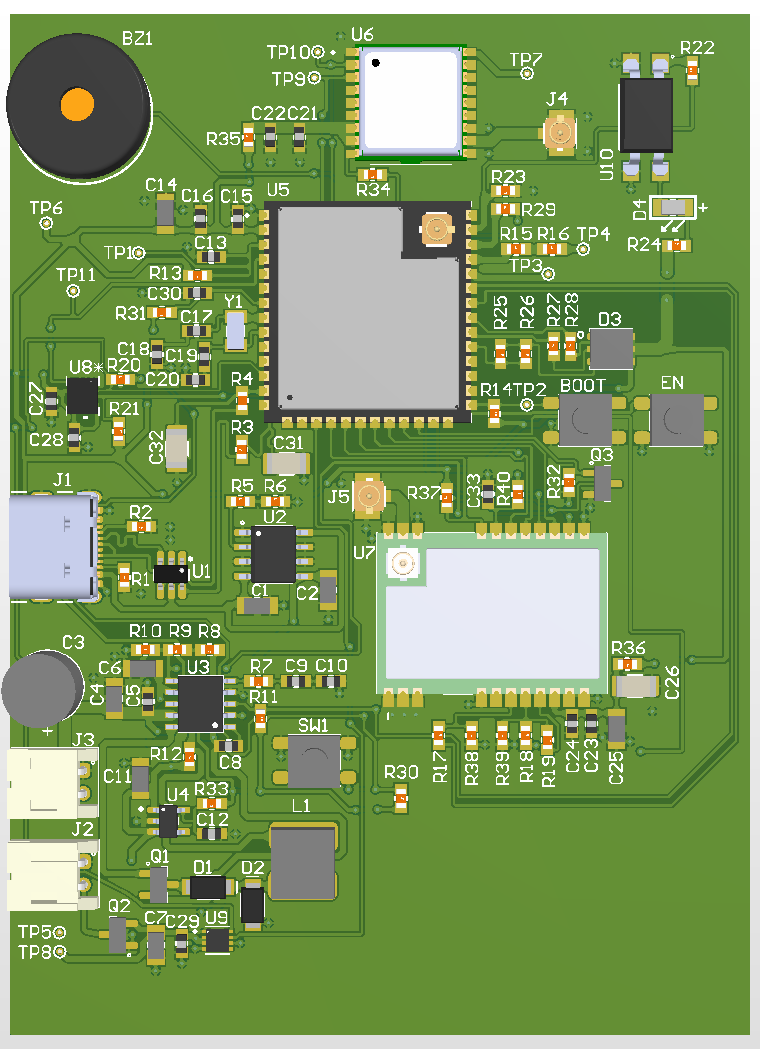
\includegraphics[height=6.7cm]{pcb_3d_top.png}};
\slideend\end{frame}

% ------------------------------------------------------------------ 2 · need
\begin{frame}[plain]\slidebegin
  \bgrect{paper}
  \eyebrow{amberdeep}{N · NECESIDAD · EL RETO DE DISEÑO}
  \slidetitle{ink}{Tres restricciones definen la placa: energía, radio y tamaño}
  \bigstat{1.1}{3.2}{4.3}{150 µA}{techo de consumo en sueño profundo (RNF-03)}{ink}
  \bigstat{5.85}{3.2}{4.3}{1–1,5 W}{de panel solar de 6 V para recargar la batería}{ink}
  \bigstat{10.6}{3.2}{4.3}{3 radios}{GNSS en 1575 MHz, LoRa en 915 MHz y Wi-Fi o BLE en 2,4 GHz, en 2535 × 3496 mil y 2 capas}{ink}
  \fill[amber] (1.1,6.55) rectangle ++(0.09,1.0);
  \txt{1.45}{6.55}{12.5}{\sz{13}{16}\bfseries}{ink}{Un collar a pleno sol y sin red eléctrica: cada microamperio y cada milímetro cuentan.}
  \footer{mute}{Fuente: nota de aplicación, secciones 1 y 3}{}
\slideend\end{frame}

% ------------------------------------------------------------------ 3 · architecture
\begin{frame}[plain]\slidebegin
  \bgrect{navy}
  \eyebrow{amber}{A · ENFOQUE · ARQUITECTURA}
  \slidetitle{cream}{La batería es el nodo central, con dos cargadores independientes}
  \bx{1.1}{3.1}{2.4}{Panel solar\\ 6 V}{}{}
  \bx{4.0}{3.1}{2.4}{\textbf{CN3791}\\ cargador solar}{}{}
  \bx{1.1}{4.55}{2.4}{USB-C\\ 5 V y datos}{}{}
  \bx{4.0}{4.55}{2.4}{\textbf{TP4056}\\ cargador USB}{}{}
  \arrowh{3.5}{3.575}{4.0}  \arrowh{3.5}{5.025}{4.0}
  \draw[fill=amber,draw=amber,rounded corners=3pt] (6.9,3.8) rectangle ++(2.0,1.2);
  \txt{7.0}{4.08}{1.8}{\sz{8}{10}\bfseries\centering}{navy}{Batería 1S\\ 3,7 V}
  \draw[-{Stealth[length=1.6mm]},amber,line width=.9pt] (6.4,3.575) -| (7.9,3.8);
  \draw[-{Stealth[length=1.6mm]},amber,line width=.9pt] (6.4,5.025) -| (7.9,5.0);
  \bx{6.9}{5.75}{2.0}{\textbf{MAX17048}\\ medidor}{}{}
  \draw[amber,line width=.9pt] (7.9,5.0) -- (7.9,5.75);
  \bx{9.4}{3.8}{1.8}{\textbf{TLV75733P}\\ LDO 3,3 V}{}{}
  \arrowh{8.9}{4.275}{9.4}
  \modbox{2.75}{ESP32-S3}{aplicación}
  \modbox{4.0}{MAX-M10S}{GNSS}
  \modbox{5.25}{DX-LR30}{LoRa}
  \modbox{6.5}{LSM6DS3TR-C}{IMU}
  \fill[amber] (1.1,7.45) rectangle ++(0.07,0.5);
  \txt{1.4}{7.47}{13}{\sz{9.5}{12}\bfseries}{cream}{El USB solo carga la batería; no alimenta el sistema.}
  \footer{steel}{Fuente: nota de aplicación, sección 2}{}
\slideend\end{frame}

% ------------------------------------------------------------------ 3b · the board
\begin{frame}[plain]\slidebegin
  \bgrect{paper}
  \eyebrow{amberdeep}{A · ENFOQUE · LA PLACA}
  \slidetitle{ink}{Cada bloque tiene su lugar en la placa}
  \node[inner sep=0pt,anchor=north west] at (1.1,2.95) {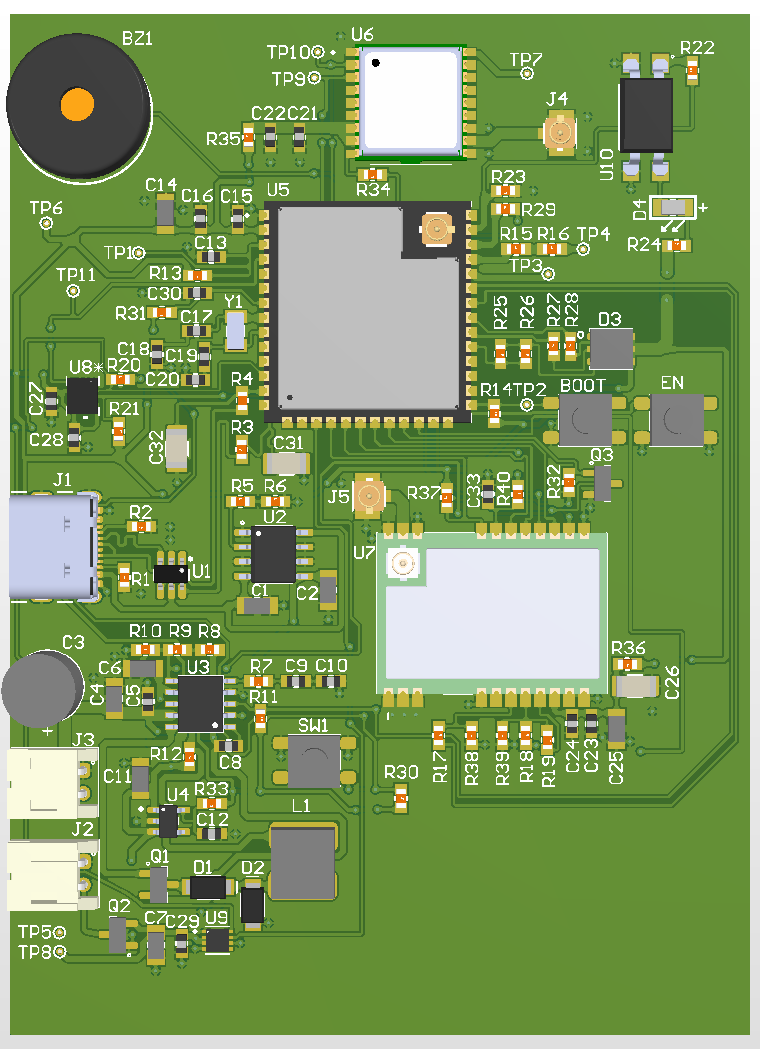
\includegraphics[height=5.0cm]{pcb_3d_top.png}};
  \pin{410}{100}{1}
  \pin{370}{305}{2}
  \pin{495}{630}{3}
  \pin{195}{700}{4}
  \pin{272}{553}{5}
  \pin{82}{395}{6}
  \legend{2.85}{1}{MAX-M10S (U6)}{Receptor GNSS multiconstelación en L1}
  \legend{3.7}{2}{ESP32-S3 (U5)}{Procesador de la aplicación}
  \legend{4.55}{3}{DX-LR30 (U7)}{Radio LoRa de 915 MHz}
  \legend{5.4}{4}{CN3791 (U3) y L1}{Cargador solar con seguimiento MPPT}
  \legend{6.25}{5}{TP4056 (U2) y USB-C (J1)}{Carga por USB y programación}
  \legend{7.1}{6}{LSM6DS3TR-C (U8)}{IMU que despierta al procesador del sueño}
  \footer{mute}{Fuente: nota de aplicación, sección 2 · vista 3D de Altium, 2535 × 3496 mil}{}
\slideend\end{frame}

% ------------------------------------------------------------------ 4 · solar
\begin{frame}[plain]\slidebegin
  \bgrect{paper}
  \eyebrow{amberdeep}{A · ENFOQUE · DECISIÓN 1 · ENERGÍA}
  \slidetitle{ink}{Un divisor de resistencias fija el punto de trabajo del panel en 6,03 V}
  \solarrow{2.95}{Punto del panel}{V = 1,205 × (1 + 400 kΩ / 100 kΩ)}{≈ 6,03 V}
  \solarrow{4.1}{Corriente de carga}{I = 120 mV / 0,47 Ω (R12)}{≈ 255 mA}
  \solarrow{5.25}{Inductancia}{L1 = 47 µH; con 10 µH no cumple}{rizado ≈ 89 mA, el 35 \%}
  \draw[fill=cardlight,draw=linelight,rounded corners=3pt] (9.7,2.95) rectangle (14.9,6.25);
  \node[inner sep=0pt] at (12.3,4.6) {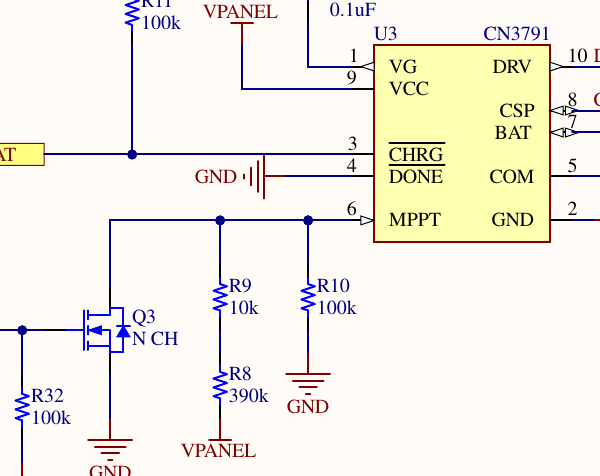
\includegraphics[height=3.0cm]{sch_1b_mppt.png}};
  \txt{9.7}{6.32}{5.2}{\sz{7}{8.5}}{mute}{Hoja 1B del esquemático: divisor R8, R9 y R10 en el pin MPPT del CN3791.}
  \fill[amberdeep] (1.1,7.0) rectangle ++(0.07,0.85);
  \txt{1.4}{7.0}{13.4}{\sz{8.8}{11}}{ink}{\textbf{Descartado:} cargar también el USB con este circuito. Con 5 V el pin MPPT no llega a 1,23 V (hace falta más de 6,15 V); por eso el USB tiene su propio cargador, el TP4056.}
  \footer{mute}{Fuente: nota de aplicación, sección 3.1}{}
\slideend\end{frame}

% ------------------------------------------------------------------ 5 · power
\begin{frame}[plain]\slidebegin
  \bgrect{navy}
  \eyebrow{amber}{A · ENFOQUE · DECISIÓN 2 · CONSUMO}
  \slidetitle{cream}{El sueño consume 124 µA, y tres piezas explican el 82 \%}
  \barrow{3.1}{MAX-M10S (GNSS)}{4.0}{46 µA}
  \barrow{3.7}{CN3791}{2.61}{30 µA}
  \barrow{4.3}{TLV75733P (LDO)}{2.17}{25 µA}
  \barrow{4.9}{IMU}{0.83}{9,5 µA}
  \barrow{5.5}{ESP32-S3}{0.70}{8 µA}
  \barrow{6.1}{MAX17048}{0.26}{3 µA}
  \barrow{6.7}{TP4056}{0.22}{2,5 µA}
  \barrow{7.3}{SX1262 (LoRa)}{0.05}{0,6 µA}
  \draw[linedark,line width=.5pt] (9.55,2.9) -- (9.55,7.85);
  \txt{9.95}{2.85}{5}{\hfont\sz{26}{28}}{amber}{≈ 124 µA}
  \txt{9.95}{3.75}{4.95}{\sz{8.5}{10.5}}{cream}{calculados, frente al techo de 150 µA. Tres piezas suman 101 µA.}
  \txt{9.95}{4.75}{4.95}{\sz{7}{9}\bfseries}{amber}{AUTONOMÍA SIN SOL · 1200 mAh}
  \autorow{5.2}{7 días}{requisito RNF-01}
  \autorow{5.8}{40–190 días}{uso normal}
  \autorow{6.4}{343 días}{techo teórico}
  \txt{9.95}{7.1}{4.95}{\sz{7.5}{9.5}}{steel}{LDO elegido: 25 µA; el descartado consume 600 µA (24 veces más).}
  \footer{steel}{Fuente: nota de aplicación, secciones 3.4 y 3.5; valores típicos de datasheet}{}
\slideend\end{frame}

% ------------------------------------------------------------------ 6 · radio and layout
\begin{frame}[plain]\slidebegin
  \bgrect{paper}
  \eyebrow{amberdeep}{A · ENFOQUE · DECISIÓN 3 · RADIO Y LAYOUT}
  \slidetitle{ink}{Tres radios conviven en dos capas: microstrip de 50 Ω y zonificación}
  \rline{3.0}{1}{Línea de 50 Ω}{Microstrip de 53 mil sobre FR4 de 31,5 mil con plano de masa continuo: de 46 a 54 Ω con la tolerancia del fabricante.}
  \rline{4.85}{2}{Criterios de ubicación}{Parche GNSS en el lado opuesto al Wi-Fi y al LoRa; lazo del cargador solar lejos del GNSS y del cristal.}
  \rline{6.55}{3}{Clases de red}{RF50 53 mil · PWR 16 mil · lazo CN3791 20 mil · USB 10 mil con longitudes igualadas.}
  \draw[fill=cardlight,draw=linelight,rounded corners=4pt] (10.0,2.85) rectangle (14.9,7.9);
  \node[inner sep=0pt] at (12.45,5.2) {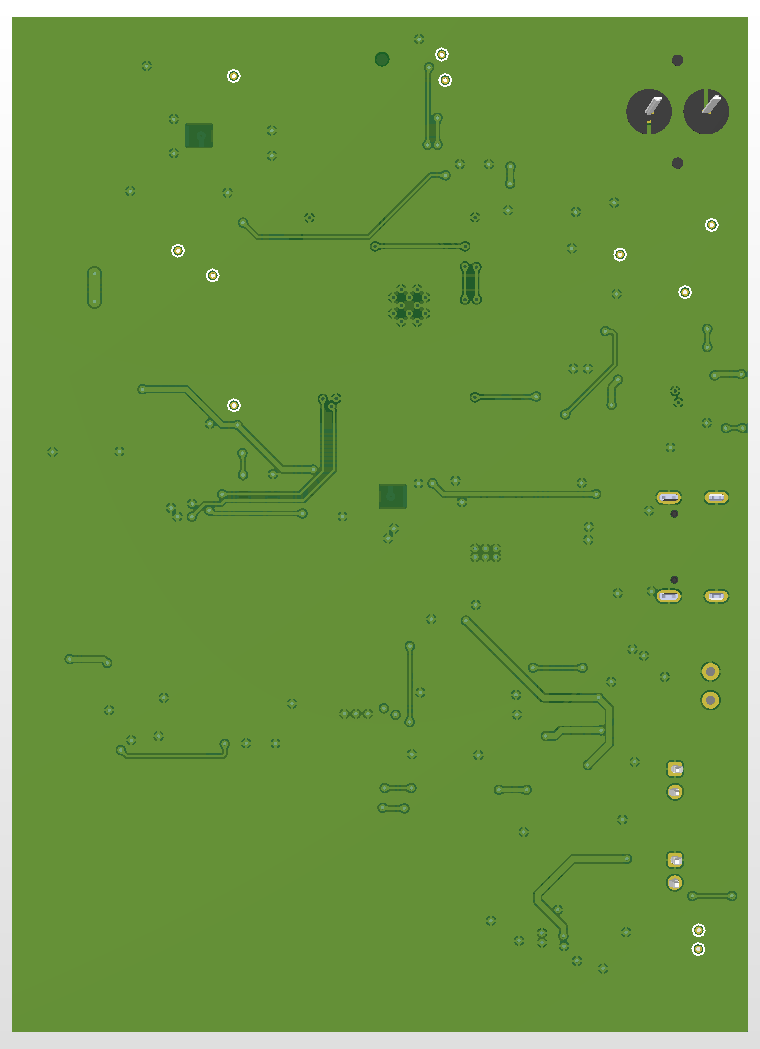
\includegraphics[height=4.2cm]{pcb_3d_bottom.png}};
  \txt{10.15}{7.38}{4.6}{\sz{6.5}{8}\centering}{mute}{Cara inferior: plano de masa continuo · 2535 × 3496 mil}
  \footer{mute}{Fuente: nota de aplicación, sección 4}{}
\slideend\end{frame}

% ------------------------------------------------------------------ 7 · firmware
\begin{frame}[plain]\slidebegin
  \bgrect{navy}
  \eyebrow{amber}{A · ENFOQUE · DECISIÓN 4 · FIRMWARE}
  \slidetitle{cream}{Un código base para dos placas: cambiar de placa es cambiar de adaptador}
  \draw[fill=amber,draw=amber,rounded corners=3pt] (1.1,3.15) rectangle ++(13.8,1.95);
  \txt{1.5}{3.4}{13}{\sz{7.5}{9}\bfseries}{navy}{COMPARTIDO}
  \txt{1.5}{3.85}{12.9}{\sz{12}{15}\bfseries}{navy}{\texttt{geofence.c} en C puro · máquina de estados · lógica de alerta · registro de eventos}
  \fwcard{1.1}{Thingy:91 X · prototipo}{GNSS dentro del módem nRF9151 y LTE-M. \texttt{geofence\_check()} tarda 350 µs con 4 vértices.}
  \fwcard{8.2}{PCB · ESP32-S3}{MAX-M10S por UART, LoRa SX1262 por SPI, IMU y medidor de batería por I2C.}
  \footer{steel}{Fuente: nota de aplicación, sección 5 · los 350 µs son de la Thingy:91 X}{}
\slideend\end{frame}

% ------------------------------------------------------------------ 8 · validation
\begin{frame}[plain]\slidebegin
  \bgrect{paper}
  \eyebrow{amberdeep}{A · ENFOQUE · VALIDACIÓN EN PROTOTIPO}
  \slidetitle{ink}{El motor de geocerca y la cadena GNSS se validaron en un prototipo}
  \midstat{1.1}{3.0}{6.5}{350 µs}{ink}
  \midcap{1.1}{3.0}{6.5}{por llamada a \texttt{geofence\_check()} con 4 vértices}
  \midstat{8.4}{3.0}{6.5}{833}{ink}
  \midcap{8.4}{3.0}{6.5}{vértices hasta los 50 ms de RF-02; con 1024 vértices, 61,4 ms}
  \midstat{1.1}{5.25}{6.5}{2,0–2,6 m}{ink}
  \midcap{1.1}{5.25}{6.5}{exactitud estimada por el receptor, caminando a cielo abierto (79 posiciones, o «fixes»)}
  \midstat{8.4}{5.25}{6.5}{54–136 s}{ink}
  \midcap{8.4}{5.25}{6.5}{hasta la primera posición válida (fix) tras un arranque en frío; tres arranques}
  \footer{mute}{Medido en el prototipo Thingy:91 X (nRF9151) · firmware: 94 268 B de flash y 19 776 B de RAM}{}
\slideend\end{frame}

% ------------------------------------------------------------------ 9 · benefit and competition
\begin{frame}[plain]\slidebegin
  \bgrect{navy}
  \eyebrow{amber}{B · BENEFICIO FRENTE AL COSTO · C · COMPETENCIA}
  \slidetitle{cream}{Cumple los 7 días sin sol y cambia el alambre por un polígono en software}
  \bccard{1.1}{Beneficio frente al costo}{Sin sol, con 1200 mAh: cumple los 7 días exigidos; de 40 a 190 estimados con uso normal}{124 µA en sueño, con recarga solar MPPT}{Precio sugerido del modelo básico: \$149.99}
  \bccard{8.2}{Cómo se resuelve hoy}{Cercas físicas: alambre y mantenimiento del perímetro}{Vigilancia con personal en el campo}{Collares comerciales de cerca virtual}
  \fill[amber] (1.1,7.2) rectangle ++(0.07,0.6);
  \txt{1.4}{7.2}{13.4}{\sz{9}{11.5}\bfseries}{cream}{Ventaja del diseño: el límite se cambia por software, el collar se recarga solo y todo el diseño está documentado de punta a punta.}
  \footer{steel}{Fuente: nota de aplicación, sección 3 · datasheet comercial (precio sugerido)}{}
\slideend\end{frame}

% ------------------------------------------------------------------ 10 · NABC close
\begin{frame}[plain]\slidebegin
  \bgrect{amber}
  \eyebrow{navy}{PROPUESTA DE VALOR · NABC}
  \slidetitle{navy}{DR-VF-01 en cuatro frases}
  \nabc{1.1}{N}{Necesidad}{Vigilar el ganado en grandes extensiones sin alambre ni red eléctrica.}{}
  \nabc{4.65}{A}{Enfoque}{Collar con GNSS, ESP32-S3 y LoRa; batería central y dos cargadores.}{}
  \nabc{8.2}{B}{Beneficio}{124 µA en sueño; 7 días sin sol exigidos y de 40 a 190 estimados.}{}
  \nabc{11.75}{C}{Competencia}{Frente a cercas físicas y vigilancia: el límite es un polígono en software.}{}
  \txt{1.1}{7.15}{13.8}{\sz{15}{18}\bfseries}{navy}{Un diseño documentado de punta a punta.}
  \footer{navy}{}{}
\slideend\end{frame}

\end{document}
